\chapter{Equal information, different topology}\label{ch:separation}

Does counting histories, or counting them together with their local neighbourhoods, tell an observer whether the history space has a hole? The answer has four layers. (i) \emph{In general no}: there are information-equivalent, topologically inequivalent pieces at every radius $\le2$ (\cref{sec:witnesses}). (ii) \emph{In the two anchor families} the history count alone suffices, because it is injective on the comparable window (\cref{sec:window}). (iii) \emph{On the six-label census} the count alone does not suffice, but radius-two histograms do, with zero residual entropy (\cref{sec:census-entropy}). (iv) That zero is a statement about collisions in a finite sample, not about prediction; \cref{sec:predictive} separates descriptive from predictive information and preserves the two predictions that failed.

\section{Information-equivalent, topologically inequivalent pieces}\label{sec:witnesses}
By a \emph{piece} we mean a content with a source whose admissible set is a single component. Two pieces are \emph{information-equivalent at radius $r$} if they have the same number of histories, the same class sizes and the same multiset of ball sizes $|B_i(w)|$ for $i\le r$.
@@prop:witnesses+computer-assisted@@
Witnesses W5 and W6 are the sharpest: radius-two data determine $N$, $E$ and $Q$ and the identity of \cref{thm:radius2} contains no hexagon term, yet these pieces differ by one hexagonal face. The combinatorial source of the difficulty is \cref{prop:petrie}: a hexagon bounding a braid face and a six-cycle bounding none cannot be told apart by the graph alone without the cube-product property.
For distinct-label pieces the fine signature through radius $3$ determines the permutohedral Betti vector in every case examined ($k=4$ with labels $\le70$, $k=5$ with labels $\le26$); whether radius three suffices in general is unknown, and radius two provably fails.

\section{The comparable window: where the count suffices}\label{sec:window}
Return to the anchors of \cref{ch:topology}: $\lambda_A=(2,3,4,5,8,9)$ with $m_0=288$ and $\lambda_B=(2,3,6,7,8,9)$ with $m_0=432$. The sources $m=m_0t$ with $t\in\{1,\dots,60\}$ realise only eight of the finite lattice of systems (\cref{prop:finite-lattice}). Let $Y_{\mathrm{anc}}$ be the anchored hole state of \cref{ch:access}.
@@obs:anchored+finite-exact@@
For $\lambda_A$ the counting law is $N(288t)=372+36[2\mid t]+72[3\mid t]+240[5\mid t]$, an injective function of the triple of indicators on the window because the increments $36,72,240$ have distinct subset sums. This is a numerical coincidence of the family rather than a mechanism; for $\lambda_B$ the non-additive $3\cdot7$ interaction ($+24$) does not destroy injectivity.

\section{The census: the count does not suffice, radius two does}\label{sec:census-entropy}
Let $\mathcal D$ be the six-label census: $8{,}008$ contents with labels in $\{1,\dots,16\}$ and $346{,}859$ regimes (distinct nonempty admissibility sets). Let $Y=\mathbf 1[\beta_2(K_A;\F)>0]$.
@@obs:equal-N+finite-exact@@
@@ex:pair+finite-exact@@
\begin{figure}[ht]\centering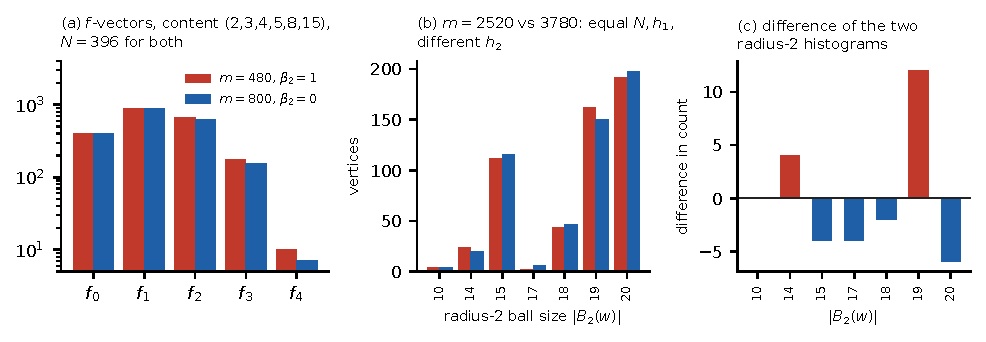
\includegraphics[width=\textwidth]{figures/fig_equal_N.pdf}
\caption{Equal history count, different topology. (a)~$f$-vectors of the pair of \cref{ex:pair} with $N=396$: the surviving hole (red) has more cells than the filled complex (blue) in every dimension $\ge1$. (b,c)~Radius-two ball-size histograms of the pair $2520$ and $3780$ at $N=540$, which have equal radius-one data; the histograms differ at a few vertices only. All values are recomputed exactly.}\label{fig:equal-N}
\end{figure}
@@thm:no-radius1+computer-assisted@@
\begin{table}[ht]\centering\footnotesize\setlength{\tabcolsep}{3pt}
\begin{tabular}{@{}lrrrrrrrr@{}}\toprule
ensemble & size & $H(Y)$ & $H(Y|N)$ & $H(Y|N,f_1)$ & $H(Y|N,\chi)$ & $H(Y|N,h_1)$ & $H(Y|f)$ & $H(Y|N,h_2)$\\ \midrule
$\mathcal E_{\mathrm{all}}$ & $346{,}859$ & $.005713$ & $.004467$ & $.002172$ & $.000109$ & $.000619$ & $0$ & $0$\\
$\mathcal E_{\mathrm{band}}$ & $93{,}018$ & $.018078$ & $.016659$ & $.008100$ & $.000406$ & $.002309$ & $0$ & $0$\\
$\mathcal E_{\mathrm{rank}}$ & $219{,}146$ & $.008231$ & $.006276$ & $.003140$ & $.000168$ & $.000803$ & $0$ & $0$\\ \bottomrule
\end{tabular}
\caption{Exact residual entropy (bits) of $Y=\mathbf 1[\beta_2>0]$ given observations, for three uniform ensembles on the census. $\mathcal E_{\mathrm{band}}$: regimes whose $N$ is attained by a positive regime. $\mathcal E_{\mathrm{rank}}$: one regime per distinct rank-indexed family mask. $f$ denotes the full $f$-vector. Plug-in values, in-sample (\cref{sec:predictive}).}\label{tab:residual}
\end{table}
@@obs:residual+finite-exact, bounded in scope@@
Two quantities are in play. The \emph{Hartley} ambiguity $\log_2N$ of a regime measures the multiplicity of its histories; the \emph{Shannon} residual $H(Y\mid\cdot)$ measures what a given observation leaves unknown about topology. They are unrelated in general: \cref{prop:witnesses} and \cref{obs:equal-N} exhibit equal Hartley and different topology, and the zero of \cref{obs:residual} exhibits zero residual with positive Hartley. The unifying fact is the ladder of \cref{thm:obs-ladder}: every observation is a function of $A$, and topology is a function of $A$ that is not a function of the cheap observations.

\section{Descriptive versus predictive information}\label{sec:predictive}
A zero residual entropy is a statement about a \emph{finite sample of signatures}. It can arise because the signature is informative, or because it is nearly injective, so that every system sits alone in its class. This section separates \emph{descriptive} information (how well the classes of a signature split positives from negatives in a sample) from \emph{predictive} information (how much a rule learned on one sample says about topology in another), and records the two statements that did not survive testing.

Let $\mathcal S$ be a finite set of systems, $Y=\mathbf 1[\beta_2>0]$ and $O$ an observation. A \emph{class} is a fibre of $O$, \emph{mixed} if it contains both values of $Y$. The \emph{plug-in} conditional entropy is computed from empirical class frequencies,
\[
H_{\mathrm{plug}}(Y\mid O)=\sum_{c}\frac{|c|}{|\mathcal S|}\,\mathrm h\!\left(\frac{|c\cap Y^{-1}(1)|}{|c|}\right),\qquad \mathrm h(p)=-p\log_2p-(1-p)\log_2(1-p).
\]
Two ensembles are used: the \emph{natural} ensemble, uniform on regimes (positives are rare, $H(Y)=0.005713$ bits on the census), and the \emph{balanced} ensemble, which weights positives and negatives equally. Both are experimental conventions, not probability laws of the grammar.
@@lem:zero-cheap+analytic@@
@@obs:separators+finite-exact@@

\subsection*{A pre-registered test}
The signatures $S_A=(N,S_{BB})$, $S_B=(Q,S_{s2})$ and $S_C=(S_{d2},S_{s2})$ were found on the census to have no mixed class. Before any held-out system was generated, the following was fixed in writing, together with sampling frame, random seeds and a hash of the feature file. A held-out set H6 of $6000$ contents was drawn uniformly from six-subsets of $\{1,\dots,22\}$ whose maximum label lies in $17$--$22$, with all regimes of each content. Prediction P1 was that each of $S_A,S_B,S_C$ has no mixed class in H6 or in the pooled set, and could be falsified by a single mixed class; P2 was that $(N,h_1)$ leaves some positive in a mixed class. An exploratory seven-label sample H7 of $120$ contents carried no prediction.
@@obs:preregistered+bounded@@
$(N,S_{BB})$ is a good fingerprint on $\mathcal D$ but not a law.

\subsection*{A general principle that is false}
After the test the question was whether $(Q,S_{s2})$ separates for a structural reason, such as every arithmetic system being prefix-defined, or only because of arithmetic closure.
@@obs:S2-falsified+finite-exact and bounded@@
@@obs:hard-positives+bounded@@

\subsection*{Descriptive versus predictive}
@@obs:plugin+finite-exact@@
@@obs:oos+bounded@@
\begin{figure}[ht]\centering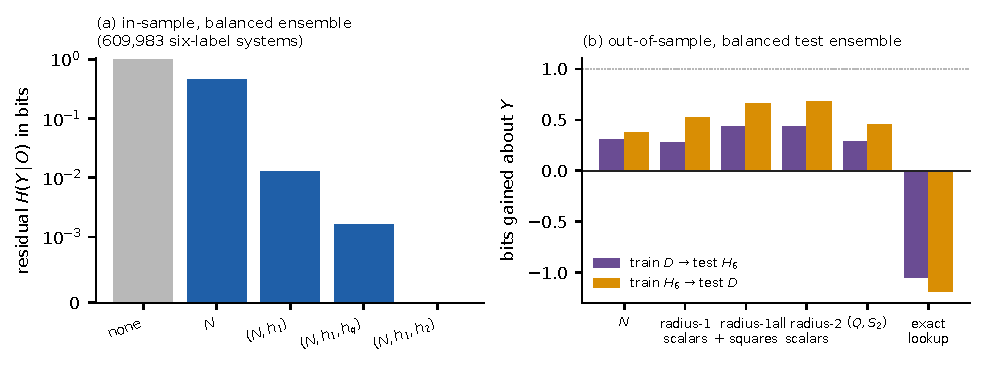
\includegraphics[width=\textwidth]{figures/fig_recovery.pdf}
\caption{(a)~In-sample residual entropy $H(Y\mid O)$ of the hole indicator by observation level, balanced ensemble on $609{,}983$ six-label systems. (b)~Information gained about $Y$ when a rule is trained on one sample and tested on the other. The in-sample residual falls to $0$ while the out-of-sample gain saturates near $0.4$--$0.7$ bits. Both panels plot values obtained in earlier computations (cf.\ \cref{app:status}); none is recomputed here.}\label{fig:recovery}
\end{figure}
@@obs:beta1-hierarchy+finite-exact@@
The two falsified statements are why the thesis of this monograph is formulated in terms of \emph{structure} (forbidden histories, locality) and not of a statistic: the statistics that work do so on the families where they were found, and the mechanism that makes them work is not known. The next chapters supply the structural mechanism that \emph{is} proved.
